La verificación funcional es una rutina de control que sirve para que el desarrollador se asegure de lo que ha descripto a través de un lenguaje de alto nivel (VHDL en este trabajo), se corresponda con el funcionamiento esperado previo a la descripción. Para efectuar esta verificación, se describe el comportamiento esperado de las señales que de entrada al circuito desarrollado, se simula el sistema y se corrobora que las salidas y se comporten conforme a lo esperado.

Para efectuar la verificación funcional de la máquina de estados desarrollada, se describió en VHDL un ciclo típico de entrada de datos desde la interfaz y se realizó un chequeo de las salidas, tanto hacia el sistema exterior, como hacia el interior. También se simuló la entrada de datos desde el FPGA, generando la rutina de salida de datos hacia la interfaz.

Debido a que es una simulación y no si implementa en físco, la declaración de la entidad se deja en blanco.
%
%\begin{lstlisting}[language=VHDL,backgroundcolor=\color{gray!30}]
%entity fx2lp_tb is
%end fx2lp_tb;
%\end{lstlisting}

En la implementación de la arquitectura, se declara e instancia el componente bajo prueba, en este caso la MEF y las señales necesarias para su correcta instanciación.

%\begin{lstlisting}[language=VHDL,backgroundcolor=\color{gray!30}]
%
%ARCHITECTURE behavior OF fx2lp_tb IS 
% 
%    -- Component Declaration for the Unit Under Test (UUT)
% 
%    component fx2lp_interface
%    port(
%         clk : in  std_logic;
%         reset : in  std_logic;
%         fdata : inout  std_logic_vector(15 downto 0);
%         faddr : out  std_logic_vector(1 downto 0);
%         slrd : out  std_logic;
%         slwr : out  std_logic;
%         flaga : in  std_logic;
%         flagb : in  std_logic;
%         flagc : in  std_logic;
%         flagd : in  std_logic;
%         sloe : out  std_logic;
%         pktend : out  std_logic;
%         send_req : in  std_logic;
%         rx_data : out  std_logic_vector(15 downto 0);
%         data_to_tx : in  std_logic_vector(15 downto 0)
%        );
%    end component;
%    
%
%   --Inputs
%   signal clk : std_logic := '0';
%   signal reset : std_logic := '0';
%   signal flaga : std_logic := '0';
%   signal flagb : std_logic := '0';
%   signal flagc : std_logic := '0';
%   signal flagd : std_logic := '0';
%   signal send_req : std_logic := '0';
%   signal data_to_tx : std_logic_vector(15 downto 0) := (others => '0');
%
%	--BiDirs
%   signal fdata : std_logic_vector(15 downto 0);
%
% 	--Outputs
%   signal faddr : std_logic_vector(1 downto 0);
%   signal slrd : std_logic;
%   signal slwr : std_logic;
%   signal sloe : std_logic;
%   signal pktend : std_logic;
%   signal rx_data : std_logic_vector(15 downto 0);
%
%   -- Definicion periodo reloj
%   constant clk_period : time := 10 ns;
% \end{lstlisting}
 
Una vez declarado e instanciado el componente bajo prueba, se generan los estímulos. De estos estímulos, las señales que emulan el reloj y el reset se establecen de forma concurrente. La señal de reloj es la que sincroniza el funcionamiento del sistema. La señal de reset es importante ya que asegura que el dispositivo inicie en el estado determinado por el diseño. 
%Se muestra en seguida, la instanciación de los componentes y la generación de reloj y reset realizadas.

%\begin{lstlisting}[language=VHDL,backgroundcolor=\color{gray!30}]
%begin
% 
%	-- Instantiate the Unit Under Test (UUT)
%   uut: fx2lp_interface port map (
%          clk => clk,
%          reset => reset,
%          fdata => fdata,
%          faddr => faddr,
%          slrd => slrd,
%          slwr => slwr,
%          flaga => flaga,
%          flagb => flagb,
%          flagc => flagc,
%          flagd => flagd,
%          sloe => sloe,
%          pktend => pktend,
%          send_req => send_req,
%          rx_data => rx_data,
%          data_to_tx => data_to_tx
%        );
%
%   --  definicion reloj y reset
%	clk <= not clk after clk_period/2;
%	reset <= '0', '1' after 100 ns;
%
%\end{lstlisting}

Finalmente, se declara el proceso que contiene los estímulos, emulando el funcionamiento de la interfaz. En un primer momento, las memorias FIFO se encuentran descargadas, es decir, los flags que indican memoria FIFO vacía se encuentran activos ({\it FLAGB} y {\it FALGD} en bajo), en tanto los flags que señalan memoria FIFO llena, se encuentran inactivos ({\it FLAGA} y {\it FLAGC} en alto).
A su vez, el bus de datos {\it FDATA[15:0]} y el de dirección {\it FADDR[1:0]} se encuentran en estado de alta impedancia (`Z') y las salidas {\it SLWR, SLRD} y {\it SLOE} se encuentran inactivas. Estas condiciones se mantuvieron hasta que se desactiva la señal de reset, y luego, se mantienen por 5 ciclos de reloj. Así, se corrobora que ante la ausencia de estímulos, el sistema se mantiene invariable.

Luego, se simula la operación de lectura de la memoria FIFO, con una serie de 3 datos aleatorios. Para este propósito, se desactivó la señal {\it FLAGB}, el flag vacío que corresponde al EP8, es decir, la memoria FIFO de salida (desde el Host). Seguidamente, se espera a la señal {\it SLOE}. Esta señal habilita a la interfaz a hacer uso del bus de datos {\it FDATA[15:0]}, por lo que se simulan datos aleatorios colocados en él, y luesgo se espera por la respuesta del sistema, el cual debería activar la señal de lectura {\it SLRD}.

Una vez realizada la operación de escritura se procede a describir la operación de escritura. Para esto, se colocó un dato en el bus de envío de datos, {\it DATA\_TO\_TX} y se activa la señal de envío de datos {\it SEND\_REQ}. Una vez que se activa la señal {\it SLWR}, se está en condiciones de cambiar el dato que se está enviando.

Se realizan también dos pruebas extra, en el desempeño de la máquina de estados desarrollada. En primer lugar, se observa la interrupción del proceso de escritura a través de la señalización del ingreso de datos. Es decir, se debe detener el envío de datos cuando la señal {\it FLAGB} se active.

Además, se observa que también se debe detener el envío de datos cuando la memoria FIFO que recibe los datos que salen de nuestro sistema se llena. Esta situación es avisada por el la interfaz a través de la señla {\it FLAGA}.

%Se muestra a continuación la descripción en VHDL de lo escrito anteriormente.
%
%\begin{lstlisting}[language=VHDL,backgroundcolor=\color{gray!30}]
%-- Process de estimulos
%stim_proc: process
%begin	
%	-- estado de reset	
%	flaga <= '1';
%	flagb <= '0';
%	flagc	<= '1';
%	flagd	<= '0';
%	send_req <= '0';
%	data_to_tx <= (others => 'Z');
%	wait until reset = '1';
%	
%	wait for clk_period*5;	
%
%		-- operacion de lectura
%		flagb <= '1';
%		wait until sloe = '0';
%
%		fdata <= x"AAAA";
%		wait until slrd = '0';	
%
%		fdata <= x"8888";
%		wait until slrd ='0';
%
%		fdata <=x"3846";
%		wait until slrd = '0';
%		--no interrupcion de lectura
%		fdata <= x"aaaa";
%		flagb <= '0';
%		wait until rising_edge(slrd);		
%		data_to_tx <= x"abcd";
%		send_req <= '1';
%		
%		--operacion de escritura
%		wait until sloe='1';
%		fdata <=(others => 'Z');
%		wait until slwr='0';
%
%		data_to_tx <= x"392a";
%		wait until slwr='0';
%
%		data_to_tx <= x"4444";
%		wait until slwr='0';
%
%		data_to_tx <= x"a8b2";
%		--interrupcion por prioridad
%		flagb <= '1';
%		wait until sloe = '0';
%		fdata <= x"1515";
%		wait until slrd='0';
%		flagb <= '0';
%		wait until sloe = '1';
%		-- operacion de escritura
%		data_to_tx <= x"2525";
%		fdata <= (others => 'Z');
%		wait until slwr = '0';
%
%		data_to_tx <= x"7868";
%		wait until slwr = '0';
%		--interrupcion por llenado de memoria
%		flaga <= '0';
%		--final de operacion escritura
%		
%		wait;
%   end process;
%\end{lstlisting}

\begin{figure}[ht]
	\centering
	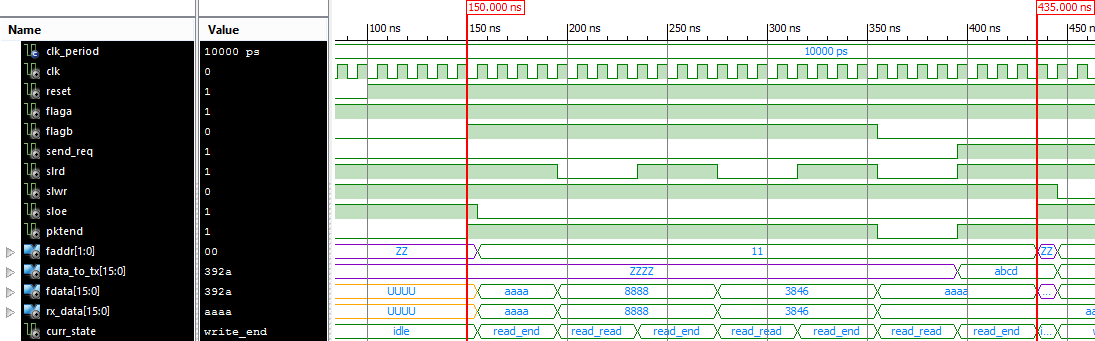
\includegraphics[width=\textwidth]{mef_tb_lect_marcas}
	\caption{Diagrama temporal de la operación de lectura entregado por el simulador}
	\label{tb:lect}
\end{figure}

Se puede observar en la Figura \ref{tb:lect} el diagrama temporal obtenido a partir de la simulación. Se resalta en este diagrama que luego de liberada la señal de reset, el sistema conserva todas las variables en el estado esperado mientras no existe estímulo.

Una vez que es desactivada la señal {\it FLAGB}, el bus de dirección apunta a la memoria FIFO de entrada de nuestro sistema, es decir, {\it FADDR[1,0]}=$''11''$. La señal {\it SLOE} se coloca en bajo, ese decir que activa el bus de datos, {\it FDATA[15:0]} para que sea usado por la interfaz. Como se indicó en la descripción realizada, se coloca un dato en el bus y este es volcado en el bus que comunica los datos que ingresan al interior del sistema, {\it RX\_DATA[15:0]}. Luego, se activa la señal {\it SLRD} en forma repetida, tal y como se espera.

También se comprueba que el estado actual en cada uno de los momentos es el adecuado. Además, se oberva que, aunque se coloquen datos en el bus de salida interno {\it DATA\_TO\_TX[15:0]} y se active la señal de envío
{\it SEND\_REQ}, el bus de datos que se comunica con la interfaz {\it FDATA[15:0]} permanece con los datos externos.

\begin{figure}[b]
	\centering
	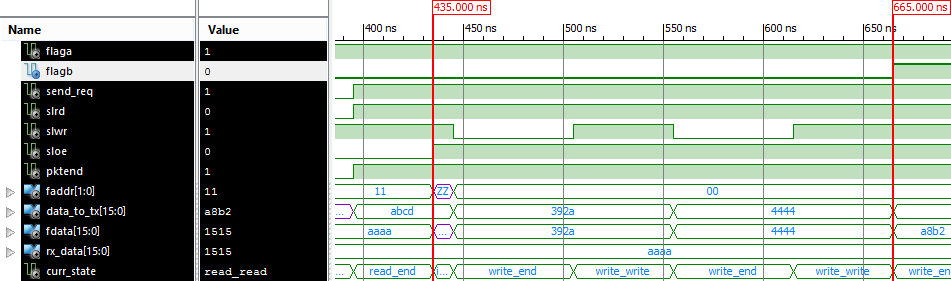
\includegraphics[width=\textwidth]{mef_tb_escr_marcas}
	\caption{Diagrama temporal de la operacion de escritura entregado por el simulador}
	\label{tb:escr}
\end{figure}

Una vez que la MEF alcanzó el estado inicial ({\it IDLE}, como se ve en la Figura \ref{tb:escr}), procede a la escritura de datos. A partir de allí, mientras no existan datos en la memoria de entrada ({\it FLAGB} permanezca en alto), la memoria de salida no se encuentre llena ({\it FLAGA} se encuentre en alto) y sea requerido el envío de datos, el sistema procede a activar en forma sistemática los datos que encuentra en el bus de envío de datos {\it DATA\_TO\_TX}.

\begin{figure}[ht]
	\centering
	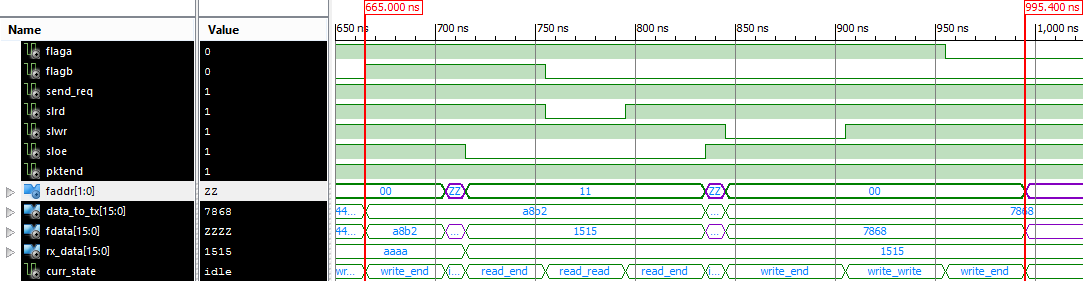
\includegraphics[width=\textwidth]{mef_tb_full}
	\caption{Diagrama temporal que muestra las interrupciones de la operación de escritura}
	\label{tb:inter}
\end{figure}

La Figura \ref{tb:inter} muestra cómo el sistema finaliza la operación de escritura cuando un sucede al menos uno de los eventos considerados para su interrupción. Cuando se activa {\it FLAGB} mientras se ejecuta la operación de escritura, esta última es interrumpida y el sistema procede a realizar, el próximo estado, la operación de lectura. En el caso de que active la señal {\it FLAGA}, indicando que la memoria que recibe los datos que envía el FPGA alcanzó el máximo de capacidad, el proceso de escritura es detenido. En ambos casos, no es relevante el valor de la señal de envío de dato {\it SEND\_REQ}, ya que ambos eventos poseen prioridad a esta.
 
Una vez realizada la simulación y verificación funcional de la síntesis desarrollada, se está en condiciones de grabar dicha síntesis en el FPGA y se puede proceder a realizar pruebas de funcionamiento más avanzadas. Las pruebas del sistema realizadas se detallan en el capítulo siguiente.

El código completo de la simulación, se pueden leer en el Anexo \ref{ap:vhdl}.